\documentclass[11pt,a4paper]{article}
\usepackage{a4wide,url,graphicx,wrapfig}
\usepackage[utf8]{inputenc}
\usepackage[ngerman]{babel}

\parindent0pt
\parskip3pt

\title{Der Mensch und das technische System} 

\author{Nikolay Shpakovsky, Minsk}

\date{20. Januar 2003}

\begin{document}
\maketitle

\begin{quote}
  Der russische Originaltext besteht aus zwei Teilen, die hier zusammengefasst
  sind
  
  Teil 1: \url{http://www.gnrtr.ru/Generator.html?pi=201&cp=3}\\
  Teil 2: \url{http://www.gnrtr.ru/Generator.html?pi=200&cp=3}
\end{quote}

\section*{Ist der Mensch Teil des technischen Systems oder nicht?}


\begin{flushright}
 \ldots{} die letzten Worte des Buches des Propheten Lustrog lauten: „alle
 wahren Gläubigen öffnen ihre Eier an dem Ende, an de es bequemer
 ist". \\ Jonathan Swift, Gulliver's Reisen. 
\end{flushright}

\section*{Einleitung}
Die Theorie des Lösens von Erfindungsaufgaben (TRIZ), vom talentierten
Ingenieur, Erfinder und genialen Ausdenker G.S. Altshuller entwickelt, ist
weit bekannt und zur heutigen Zeit zweifellos das wirksamste Werkzeug zur
Lösung von Ingenieuraufgaben. Eine große Zahl von Materialien ist dazu in
Russisch und Englisch veröffentlicht worden, in denen das Wesen der Theorie
für eine erste Einführung ausreichend umfassend dargestellt wird.  Die beste
russischsprachige Ressource ist die Website des Minsker
OTSM-TRIZ-Zentrums\footnote{\url{http://www.trizminsk.org}}, die bestes
Englischsprachige der Amerikanische
TRIZ-Journal\footnote{\url{http://www.triz-journal.com}}. Wenn man TRIZ aus
Büchern und Artikel studiert hat, kann man leicht andere unterrichten -- das
Material ist so reichhaltig und faszinierend, dass das Interesse an einer
Beschäftigung mit dem Stoff gewährleistet ist.

Für ein tieferes Verständnis der TRIZ ist jedoch eine sorgfältige Abwägung des
vorgestellten Materials erforderlich, vor allem der Konzepte und Begriffe der
TRIZ.  Vieles in TRIZ ist als Material zur Anregung zum weiteren Nachdenken
beschrieben und nicht als Menge von Informationen zum einfachen
Auswendiglernen.

Als ich für SAMSUNG als TRIZ-Berater arbeitete, musste ich alles, was ich
bisher über die TRIZ wusste, von neuem und ernsthaft überdenken. Bei der
Lösung technischer Aufgaben, der Umgehung von Patenten konkurrierender
Unternehmen und der Erarbeitung von Prognosen der Entwicklung technischer
Systeme war es sehr wichtig, den tieferliegenden Inhalt jedes Begriffs der
TRIZ genauer zu verstehen, um die TRIZ-Instrumente mit maximaler Effektivität
anzuwenden.

Eines der grundlegenden Konzepte in der TRIZ und eines der wichtigsten
Bindeglieder aller seiner Instrumente ohne Ausnahme ist der Begriff
„Technisches System“. Dieser Begriff wird in der klassischen TRIZ ohne
Definition eingeführt, als Ableitung des Begriffs „System“. Aber bei näherer
Betrachtung wird klar, dass dieser Begriff -- „Technisches System“ -- eine
weitere Konkretisierung erfordert. Zu Gunsten einer solchen Behauptung spricht
zum Beispiel der semantische Aspekt. Der Begriff „technisches System“ wird auf
zwei Arten vom Russischen ins Englische übersetzt: „Tecnical System“ und
„Engineering System“.  Mit einer beliebigen Suchmaschine im Internet kann man
sich leicht überzeugen, dass diese beiden Konzepte von Fachleuten, die in der
TRIZ aktiv sind, fast gleichwertig verstanden werden. Oder nehmen Sie zum
Beispiel das Glossar von Victor
Fey\footnote{\url{http://www.triz-journal.com/archives/2001/03/a/index.htm}}},
  in dem einfach keines der beiden Konzepte erläutert wird.

In diesem Artikel habe ich versucht, mein Verständnis des Begriffs
„technisches System“ zu beschreiben, das sich schrittweise entwickelt hat,
wenn ich zur Lösung einer konkreten Aufgabe die vollständige Zusammensetzung
eines minimalen technisch arbeitsfähigen Systems herausfinden musste.

\section*{Ein Versuch, den Begriff „technisches System“ zu analysieren}

Lasst uns zunächst einmal überlegen, was ein System überhaupt ist. Es gibt
viele verschiedene Systemdefinitionen. Die einprägsamste, abstrakteste, und
damit absolut erschöpfende Definition, die aber von geringem praktischen
Nutzen ist, hat B. Gaines [1] gegeben: \textbf{„Ein System ist das, was wir
  als ein System definieren“}.  In der Praxis wird die Systemdefinition von
A. Bogdanov am häufigsten verwendet [2]: \textbf{"Ein System ist eine Menge
  miteinander verbundener Elemente mit einer gemeinsamen (System-)Eigenschaft,
  die nicht auf Eigenschaften dieser Elemente reduzierbar ist“}.

Was aber ist ein "Technisches System"? 

Leider ist das Konzept des „Technischen Systems“ bei G. Altschuller nicht
direkt definiert. Aus dem Kontext wird klar, dass es sich um eine Art System
handelt, das mit Technik technischen Objekten zu tun hat. Als indirekte
Definition eines technischen Systems (TS) können drei von Altschuller
formulierte Gesetze oder vielmehr drei Bedingungen dienen, die für deren
Existenz erfüllt sein müssen [3]:
\begin{itemize}
\item[1.] Das Gesetz der Vollständigkeit der Teile des Systems. 
\item[2.] Das Gesetz der „Energieleitfähigkeit“ des Systems. 
\item[3.] Das Gesetz der Abstimmung der Rhythmik der Teile des Systems.
\end{itemize}
Nach dem Gesetz der Vollständigkeit der Teile des Systems umfasst jedes TS
mindestens vier Teile: Antrieb, Transmission, Arbeitskörper und
Steuerungssystem.
\begin{center}
 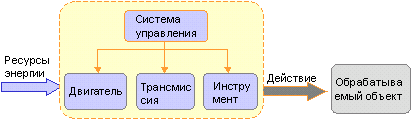
\includegraphics[width=.6\textwidth]{mts-1.png}\\ Minimale Struktur eines
 funktionsfähigen technischen Systems nach G. Altschuller.
\end{center}
Das heißt, es gibt ein System, eine Maschine, die aus technischen Objekten,
Untersystemen besteht, das die geforderte Funktion erfüllen kann. Es umfasst
wenigstens das Arbeitsorgan, die Transmission und den Antrieb. Alles, was den
Betrieb dieser Maschine steuert, wird im „Steuerungssystem“ oder dem
unverständlichen „kybernetischen Teil“ [4] zusammengefasst.

Wichtig ist hier das Verständnis, dass das TS geschaffen wurde, um eine
bestimmte Funktion auszuführen. Wahrscheinlich sollte das so verstanden
werden, dass ein minimal funktionsfähiges TS diese Funktion zu jeder Zeit
ausführen kann, ohne zusätzliche Ergänzungen. Ansätze zur Definition eines
technischen Systems werden in dem Buch „Suche nach neuen Ideen“ [5]
vorgestellt, wo eine Definition eines „sich entwickelnden technischen Systems“
gegeben wird. Diese Frage wird von V. Korolev in seinen interessanten Studien
[6,7] aufgegriffen. Einige kritische Anmerkungen dazu sind in den Materialien
von N. Matvienko [8] zu finden. Die Definition des Begriffs „technisches
System“ selbst bezogen auf die TRIZ wird in dem Buch [9] von Yu. Salamatov
beschrieben: 
\begin{quote}\bf
  Ein technisches System ist eine Menge geordnet interagierender Elemente mit
  Eigenschaften, die nicht auf die Eigenschaften einzelner Elemente
  zurückzuführen sind, und die dazu bestimmt ist, bestimmte nützliche
  Funktionen zu erfüllen. 
\end{quote}
In der Tat hat der Mensch irgendwelche Bedürfnisse, zu deren Befriedigung
irgendeine Funktion ausgeführt werden muss. Das heißt, man muss irgendwie ein
System organisieren, das diese Funktion ausführt -- das „Technische System“ --
und das Bedürfnis zu befriedigen.

Was verwundert an der obigen Definition des technischen Systems? Die nicht
ganz klare Wendung „ist bestimmt für“. Wahrscheinlich sind hier nicht die
Wünsche von irgendjemandem wichtiger, sondern die objektive Fähigkeit, die
geforderte Funktion zu erfüllen.  
\begin{quote}\it
  Wozu dient zum Beispiel ein Metallzylinder mit einer axialen Bohrung mit
  variablem Durchmesser und Gewinde an einem Ende?

  Es ist praktisch unmöglich, diese Frage zu beantworten. Die Diskussion
  verschiebt sich sofort auf die Ebene der Frage „wo könnte man das
  anwenden?“.
\end{quote}
Aber kann man, wenn man diese Definition benutzt, sagen: das ist noch kein
Technisches System, aber von diesem Moment an -- nun ist es ein Technisches
System? Es heißt dazu wie folgt: "... ein TS erscheint, sobald ein technisches
Objekt die Fähigkeit erlangt, die Nützliche Hauptfunktion ohne den Menschen
auszuführen“. Und weiter heißt es, dass einer der Tendezen der Entwicklung TS
die Entfernung des Menschen aus dem TS ist. Das heißt, auf irgendeiner Etappe
der Entwicklung des TS ist der Mensch Teil davon. Oder nicht?
Nicht verständlich ...  
\begin{quote}\it
  Wahrscheinlich werden wir nichts verstehen, wenn wir auf die folgende Frage
  keine Antwort finden: Ist der Mensch Teil des technischen Systems oder
  nicht?
\end{quote}
Wenn ich bekannte TRIZniks befrage, erhalte ich eine ziemlich breite Palette
von Antworten: von einem entschiedenen „Nein“, unterstützt durch Hinweise auf
Koryphäen, bis zu einem zögerlichen „Ja, wahrscheinlich“.

Die originellste der Antworten: Wenn sich ein Auto gleichmäßig und geradlinig
bewegt, dann ist der Mensch nicht Teil dieses technischen Systems, aber sobald
das Auto beginnt, um eine Kurve zu fahren, so wird der Mensch sofort sein
notwendiger und nützlicher Teil.

Was haben wir dazu in der Literatur? Salamatov [9, Abschnitt 4.3] gibt ein
Beispiel, in welchem ein Mann mit der Hacke kein TS ist. Zumal die Hacke
selbst auch kein Technisches System ist. Aber Pfeil und Bogen sind ein TS.

Aber was ist der Unterschied zwischen einer Hacke und einem Bogen? Der Bogen
haben einen Energiespeicher - die Bogensehne und eine flexible Stange, bei
einer guten Hacke biegt sich der Stiel ebenfalls beim Schwingen, was beim
Abwärtsbewegen die Stoßkraft erhöht. Sie biegt sich nur ein wenig, aber uns
geht es ums Prinzip. Mit dem Bogen wird in zwei Phasen gearbeitet: Zuerst
spannen, dann loslassen -- mit einer Hacke auch. Warum dann so eine
Ungerechtigkeit?

Versuchen wir es herauszufinden. 

Ist ein angespitzter Holzstab ein technisches System? Es sieht nicht danach
aus.  Ein Kugelschreiber? Wahrscheinlich ein TS, und ein ziemlich
kompliziertes. Und ein Drucker?  Zweifelsohne ein TS.

Und einen Bleistift? Wer weiß ...? Wohl so: sowohl als auch. Vielleicht
sollten wir ihn "Einfaches Technisches System" nennen? Ein Schreibgriffel aus
Blei oder Silber? Eine Frage ...  Kein einfaches Holzstück mehr, es ist
immerhin aus einem edlen Metall, aber bis zum Kugelschreiber ist es noch weit.

Ein moderner Kapillarschreiber, ein Bleistift, ein angespitzter Stab und der
Schreibkopf eines Druckers, was haben sie gemeinsam? Eine gewisse nützliche
Funktion, die sie im Prinzip ausführen können: „eine Spur auf einer Oberfläche
hinterlassen“.

„Der langlebige Timoschka läuft auf einem schmalen Pfad. Seine Fußabdrücke
sind Ihre Werke“. Erinnern Sie sich an dieses Rätsel? Gemeint ist ein
Bleistift.  Aber auch ein Stock, ein Schreibgriffel aus Blei oder Silber, ein
Stift, Marker, Drucker, eine Druckerpresse. Was für eine Auswahl! Und die
Reihung ist logisch ...

Wirklich, es stellt sich wieder eine Frage. 

Wenn alle diese Objekte die gleiche Funktion erfüllen können, dann sind das
alles -- Technische Systeme. Und mann muss Sie nicht in komplizierte und
primitive unterteilen. Wenn Objekte die gleichen Funktionen erfüllen, dann
dienen sie nur demselben Zweck, sondern auch die Hierarchieebene muss dieselbe
sein.

Oder umgekehrt, es sind alles keine TS. Nun, was ist das auch für ein
Technisches System -- ein angespitzter Stock? Wo ist der Antrieb oder die
Transmission?  Aber dann kommt heraus, dass der Drucker auch kein TS ist.

Lassen Sie uns formal vorgehen. 

Jedes Technische System muss irgendeine nützliche Funktion erfüllen.
Kann ein angespitzter Stock seine Funktion erfüllen? Nein. Und der Drucker?

Lassen Sie uns einen einfachen Versuch machen. Wir legen den Stift auf den
Tisch. Oder, der Einfachheit halber auf Papier.  Und nun warten wir einfach,
bis er anfängt, seine nützliche Hauptfunktion zu erfüllen.  Macht er nicht.
Und macht es so lange nicht, bis der Mensch, der Operator, ihn nicht in die
Hand nimmt und damit das Blatt Papier berührt, und „... die Gedichte fließen
fre aus der Feder“.

Und der Drucker? Beginnt er mit dem Drucken, bevor nicht der Benutzer den
Befehl an den Computer gegeben hat, und dieser den Befehl nicht seinerseits an
den Drucker weitergeleitet hat? Also, ohne das Drücken einer Taste, eines
Sprachbefehls oder, perspektivisch, eines Gedankenbefehls wird die Aktion
nicht stattfinden.

Damit ergibt sich folgendes. Stift, Hacke, Drucker, Fahrrad sind keine TS.
Genauer, keine vollständigen TS. Es sind nur „Systeme technischer Objekte“.
Ohne Menschen als Operator können sie nicht arbeiten, d.h. können sie ihre
Funktion nicht erfüllen. Natürlich, im Prinzip können sie es, aber in der
Realität ... Auf die gleiche Weise können vier Räder, Karosserie und
Motorhaube nichts irgendwohin transportieren ... Nicht einmal ein voll
ausgestatteter Neuwagen, vollgetankt, mit Schlüssel im Zündschloss ist ein
technisches System, sondern einfach ein „System technischer Objekte“.  Wenn
sich der Operator -- in gewöhnlicher Sprache auch Chauffeur genannt -- auf
seinen Platz setzt und das Lenkrad erfasst, sofort wird das Auto zu einem
Technischen System. Und all die anderen technische Objekte und Systeme werden
vollständige TS und funktionieren nur und ausschließlich mit einem Menschen,
einem Operator.

Der Operator kann innerhalb des „Systems technischer Objekte“ sitzen. Er kann
daneben stehen, entfernter oder näher. Kann überhaupt nur die Aktion des
Technischen System programmieren, es einschalten und weggehen. Aber in jedem
Fall muss der Betreiber sich an der Verwaltung des TS beteiligen.

Und es ist nicht nötig, ein Raumschiff und eine Hacke einander
entgegenzustellen. Wie das erste so ist auch die zweite ein größerer oder
kleinerer Teil eines TS, das für die normale Ausführunge der nützlichen
Hauptfunktion durch einen oder mehrere Betreiber ergänzt werden muss.

Erinnern wir uns an das Gesetz der Vollständigkeit der Teile eines Systems,
das von G.S. Altschuller formuliert wurde. Ein TS entsteht dann, wenn alle
vier Teile davon vorhanden sind (Abb. 1), wobei jedes von ihnen minimal
arbeitsfähig sein sollte. Wenn auch nur ein Teil fehlt, handelt es sich nicht
um ein Technisches System. Genauso ist es kein TS, wenn einer der vier Teile
nicht funktionsfähig ist.  Wir erhalten damit, dass ein Technisches System
vorliegt, wenn es vollständig bereit ist für die sofortige Ausführung seiner
nützlichen Hauptfunktion ohne zusätzlichen Komplettierung. Wie ein Schiff, das
bereit ist zum Auslaufen. Alles betankt, beladen und die gesamte Besatzung auf
ihren Plätzen.

Ohne Menschen ist das Kontrollsystem nicht etwas, das „minimal funktionsfähig“
ist, sondern im Prinzip nicht funktionsfähig, weil nicht komplett. Das Gesetz
der Vollständigkeit der Teile des Systems ist nicht erfüllt. Und das Gesetz
der Energiedurchleitung ist nicht erfüllt. Geht ein Signal an das Steuersystem
und -- Stopp. Kein umgekehrter Energiefluss.

Und was machen wir mit den „Technischen Systemen“, die glücklich ihre
nützliche Funktion erfüllen, aber überhaupt keine technischen Objekte
enthalten?  Etwa der Elektriker, der eine Glühbirne auswechselt ...?

Es scheint, dass es eine besondere Hierarchieebene gibt, auf der sich die
Menge der Objekte, Elemente in ein Technisches System verwandelt. Das ist die
Ebene des Autos mit Fahrer, der Videokameras mit Kameramann, des Stifts mit
Schriftsteller, einer automatisierten Produktionsanlage mit Operatoren, die
diese in Betrieb nehmen und warten etc. Das ist also die Ebene, auf der ein
System gebildet wird: eine Menge natürlicher und technischer Objekte, der
menschliche Operator und seiner Handlungen, dass irgendeine für den Menschen
unmittelbar nützliche Funktion ausführt.

Es ist interessant zu sehen, wie die Hierarchie der biologischen Objekte und
Systeme strukturiert ist. Moleküle, Zellen, Elemente, Teile von Organismen
bilden die Ebenen der Teilsysteme.  Ein „Teilsystem“ ist ein separater Teil
des Organismus, wie das Skelett eines Elefanten, ein Mückenrüssel oder eine
Meisenfeder. Die Summe solcher Subsysteme, sogar ihr gesamtes Spektrum, ein
aus ihnen zusammengesetzter ganze Körper, kann keine nützlichen Funktionen
vollbringen.  Wir müssen diesem „Set“ noch etwas hinzufügen, den „Funken
Gottes“ einhauchen, um einen lebenden, funktionierenden Organismus zu
erhalten.
\begin{center}
 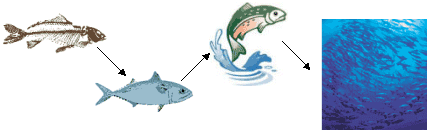
\includegraphics[width=.6\textwidth]{mts-2.png}
\end{center}

Lebende Organismen, Individuen, können sich in einem Obersystem vereinen.
„Obersystem“ ist eine mehr oder weniger organisierte Gruppe von Tieren oder
Pflanzen, zum Beispiel, ein Bienenstock. Aber ein scharfer
qualitativen Sprung geschieht hier schon nicht mehr. 

In Analogie zu biologischen Systemen können wir den Begriff "technisch"
interpretieren System" als eine besondere Hierarchieebene, auf der dem System
die Möglichkeit gegeben wird unabhängig zu handeln, d.h. auf der Ebene eines
lebenden Organismus.


Mit anderen Worten, das "technische System" in der Technik entspricht dem Niveau der
des Organismus in der Natur. In einer Patentanmeldung wird sie als "Maschine in
zu arbeiten". Das heißt, "das System der technischen Objekte" plus ein menschlicher Operator. Zum Beispiel,
ein Vergaser ist kein CU, es ist nur ein System, ein Satz technischer...
von Objekten. Und der Mann, der den Vergaser auf die Nuss klopft, ist der CU mit dem...
eine nützliche Funktion: die Nüsse von den Schalen zu reinigen. Genauso wie ein Mann mit einer Hacke - CU.
einen Traktor mit einem Pflug - nein. Paradoxon....

\mph{"Mensch" - was ist das in Anwendung auf das technische System? Was daran schwierig ist.
zu verstehen? }

Vielleicht wird die Verwirrung durch den Wortlaut der Frage selbst verursacht. Psychologisch .
Es ist schwer, einen Mann und eine Bremsbacke auf die gleiche Stufe zu stellen.

Es besteht kein Zweifel daran, dass der Mensch als Teil der Technosphäre am direktesten verwandt ist mit
eine beliebige CU und kann in den folgenden Rollensituationen in Beziehung zu ihr stehen:

\...im Supersystem. 
\begin{itemize}
\Posten[1.] von einem Benutzer. 
\Posten[2.] Entwickler. 
\Position[3.] Hersteller der technischen Objekte des Systems. 
\Posten[4.] Person für Wartung, Reparatur und Entsorgung
 der technischen Einrichtungen des Systems. 
\end{itemize}
\mph{System:} 
\begin{itemize}
\Position[1.] Bediener, Hauptbedienelement. 
\item[2.] Energiequelle. 
\item 3: Motor. 
\item[4.] Übertragung. 
\Posten[5.] Arbeitsgremium. 
\item[6.] Verarbeitetes Objekt. 
\end{itemize}
In der Umwelt:\mph 
\begin{itemize}
\Standteil[1.] Element der Umwelt. 
\end{itemize}
Der Benutzer ist zweifelsohne die Hauptperson. Er ist derjenige, der für die Gründung der CU bezahlt,
Es ist sein Wille, dass die Entwickler und Hersteller übernehmen. Er bezahlt dafür.
Betreiberarbeiten, technische Wartung, Reparatur und Entsorgung
der Systemobjekte.

Die zweite Personengruppe sorgt für das Funktionieren der CU bei der Arbeit, erlebt sie
die Handlung an sich selbst.

Die dritte Gruppe hilft oder behindert diesen Prozess indirekt, oder einfach
beobachtet sie und ist den Nebenwirkungen von
zu arbeiten.


Eine Person kann mehrere Rollen gleichzeitig ausüben. Zum Beispiel der Fahrer
Ihr eigenes Auto oder eine Person, die einen Inhalator benutzt. oder .
ein Radfahrer. Er ist ein Element fast aller Fahrradsysteme mit Ausnahme des Arbeitskörpers...
(Sitze) und Getriebe (Räder und Fahrradrahmen).


\In Ordnung, es stellt sich heraus, dass der Mensch ein obligatorischer Teil der Technischen
Systeme.}

Man sollte meinen, das würde einen Unterschied machen. Denn wenn es darum geht, reale Dinge zu lösen.
von technischen Problemen, dann geht die Person schnell an die Klammern des Problems und arbeitet.
liegt auf der Ebene des Subsystems. Ja, aber nur dort, wo Harmonisierung und...
Der Energiedurchgang erfolgt zwischen Subsystemen, die in keiner Weise verbunden sind mit
als Betreiber. Und sobald wir uns dem Kontrollsystem nähern, ist das Problem...
die Interaktion zwischen Mensch und technischen Objekten läuft auf Hochtouren.

Nehmen Sie zum Beispiel das Auto. Das Auto hat sein heutiges Aussehen bereits erhalten durch
in den späten 1970er Jahren, als die Airbags erfunden wurden und zuverlässig
Automatikgetriebe. Die meisten Verbesserungen seit dieser Zeit.
zielen nur darauf ab, Management, Sicherheit und Komfort zu verbessern.
Wartung und Reparatur, - d.h. die Interaktion des Menschen, der den Hauptteil der CU ausmacht,
mit ihren anderen Teilen.

Der Lastwagen der 40-50er Jahre hatte ein Lenkrad mit einem Durchmesser von 80 cm. Der Fahrer muss
sehr stark zu sein, um ein solches Auto zu fahren. Und in der Luftfahrt...
Ein Riesenflugzeug aus den 30er Jahren "Maxim Gorky". Um das Manöver durchzuführen, für
Das Ruder hätte den ersten und zweiten Piloten zusammenziehen müssen. Manchmal riefen sie
um dem Navigator und dem Rest der Besatzung zu helfen. Der Betreiber verwendet jetzt Verstärker
kann viel stärker belastete Mechanismen steuern. Es scheint, dass das Problem
es ist erledigt. Ah nein, man vergisst oft wieder einen Mann... Die Sache ist die, die Verstärker...
erlauben es dem Bediener nicht immer, das Verhalten des Kontrollierten vollständig zu spüren.
eines Mechanismus. Manchmal führt es zu Unfällen.


Zum Beispiel ein Autosicherheitsproblem oder ein "eintönigeres" Problem in der
an die Lokomotivsteuerung. Es ist hier sehr wichtig, dass der Operator immer in...
wach, funktionsfähig. Auch dieses Problem wird im Supersystem gelöst...
die Ursachen für das Einschlafen am Steuer beseitigt werden und eine medizinische Überwachung durchgeführt wird,
die Verantwortung des Fahrers und Betreibers steigt. Aber es wird zunehmend angesprochen.
direkt im Tech System. Direkt im Cockpit. Wenn der Maschinenbediener pünktlich ist.
wird die Alarmleuchte nicht ausgeschaltet, die Lokomotive hält an, und der Zug hält an.
wird aufhören. Oder im Auto: Man fährt erst, wenn man sich angeschnallt hat. Ich meine, jetzt kommt es.
normales Feedback, sowie zwischen allen anderen Elementen der CU.


Vielleicht ist einer der Gründe dafür, dass dies eine Richtung der Verbesserung ist
technische Systeme haben erst in den letzten Jahren begonnen, sich aktiv zu entwickeln.
ein Missverständnis des menschlichen Platzes in ihrer Struktur. Oder besser gesagt, nicht dieses Missverständnis,
und.... trotzdem gerät der Entwickler in eine komplizierte psychologische
Situation. Eine Person, die neue Dinge entwickelt, fühlt sich wie ein Schöpfer. Er hat nicht
kann das Gefühl haben, dass ein und dieselbe Person auch...
durch den Bediener, Motor oder Arbeitskörper - Teil des Mechanismus, Maschine,
Technische Systeme. Okay, wenn es sich um ein weit verbreitetes TC handelt, ist es eng.
die mit einer Person interagieren, wie ein Auto. Hier kann eine Person
gleichzeitig Entwickler, Betreiber und Benutzer zu sein.

Genau wie mit dem Computer. Es ist schwierig, mit den meisten Computerprogrammen zu arbeiten, selbst
jetzt, da die Entwickler die einfache Wahrheit gelernt haben, dass das Programm
als menschlicher Operator arbeiten, der sich um das Ergebnis kümmert, nicht um das Gerät.
Programme. Jetzt gibt es solche Begriffe wie "freundliche Schnittstelle".
Und davor... Warum weit gehen, denken Sie an "Lexikon".

Und die andere CU, die auf den ersten Blick weit entfernt von einem Mann.... namens Legion steht.
Oft kommt es mir gar nicht in den Sinn, dass eine Person ein Teil von
Technische Systeme. Und wenn man sie entwickelt, ist es notwendig
die Interaktion von Bestandteilen nach ihrer Kapazität zu querschnittlich darstellen
des menschlichen Körpers und Geistes. Manchmal wird es nicht gemacht.

Darüber hinaus werden viele der derzeit bekannten natürlichen Faktoren oft ignoriert,
die das Wohlbefinden der Person, die Klarheit ihrer Bewegungen und die Reaktionsgeschwindigkeit beeinflussen. А
neu entdeckte psychologische Faktoren, wie der "Kassandra-Effekt" [10]?

Und erhebt sich ein furchterregender Tschernobyl-Pilz, Flugzeuge stürzen ab und Schiffe kollidieren. 

\mph{Und was brauchen Sie außer einem Operator noch, um sich betriebsbereit zu machen?
Das technische System?}

Darüber - im zweiten Teil dieses Artikels.

\neue Seite
\Anfang{Zitat}
\und Zitat

\section*{Vollständiges, mindestens funktionsfähiges technisches System.]

Es gibt eine Reihe von technischen Objekten, die in das System integriert sind
Mann-Operator. Reicht es aus, wenn das Tech System
nützliche Funktion und befriedigen das Bedürfnis des Benutzers, oder brauchen etwas.
mehr?


Erinnern wir uns an das berühmte Trizovianische Beispiel aus dem Buch von G. Ivanov...
[11]. Es geht um den russischen Wissenschaftler Kapitse, der das Simmens-Werk und das Kapitse-Werk besucht hat.
Shukkerta soll Generatoren produzieren. Die Eigentümer der Anlage zeigten ihm den Generator,
der nicht arbeiten wollte und 1.000 Mark zur Korrektur anbot. Kapitsa schnell.
klatschte ab, dass das Zentrallager geneigt und verklemmt war, griff zum Hammer und schlug darauf ein.
auf dem Lagerkörper - der Generator läuft.

Verwirrte Kunden baten um eine Rechnung für die geleistete Arbeit. Kapitsa
schrieb: \mph{"1 Treffer mit dem Hammer - 1 Markierung für das Wissen, wo man treffen muss - 999.
Stempel.}


Und hier ist ein weiteres Beispiel von Phoenix Cooper [12].

Die Helden der Geschichte rannten vor der Verfolgungsjagd davon, die Indianer jagten sie in das Dickicht des hohen Trockenen.
die Kräuter und zündete sie an. Da ist eine Wand aus Feuer, was sollen wir tun? Ein alter Jäger hat nicht
wurden verwirrt und steckten das Gras in der Nähe ihres Standes in Brand. Die Brandmauer ist eingestürzt.
zu dem Feuerschacht, der sie angegriffen hat, und verbrannte Brennstoff für ihn. Feuer .
Aussterben, die Flüchtlinge wurden gerettet.

Was ist das technische System in dem einen und in dem anderen Fall?

Im ersten Beispiel. Der Benutzer muss den Generator starten. Nützlich .
Funktion ist die Ausrichtung des Lagers. Operator - Kapitsa, System technischer Objekte
- Hammer.

Es stellt sich heraus, dass das technische System ein Hammerhead-Kapitän ist.

Im zweiten Beispiel. Der Benutzer muss das Feuer stoppen. Nützlich .
Die Funktion besteht darin, das Gras zu zerstören (Brennstoff für das kommende Feuer). Betreiber - alt
Jäger, System von technischen Objekten - Feuerstein und Feuer.

Technisches System - Jäger mit Feuerstein und Feuer.

Was geht hier also vor sich? Eine vernachlässigbare Aktion von Mensch und Operateur mit Hilfe von
der primitiven technischen Mittel ein so großartiges Ergebnis wie im ersten Fall,
und der zweite Fall! Ist das alles? Ist das nicht die vollständige Ergänzung der technischen
Systeme, die es im ersten Fall ermöglichten, eine riesige
den Generator, und in der zweiten, die Feuerwand stoppen?

Nein, ist es nicht.

Das Wichtigste ist das, was in den letzten Jahren völlig übersehen wurde.
der Argumentation, ist eine Informationskomponente.

Wirklich, man kann morgens mit einem Hammer auf den Generator schlagen, bis...
der Nacht. Und Kapitsa hat nicht angeklopft, sondern auf eine streng definierte Weise. Und darin.
In diesem Fall bestand die Informationsunterstützung für seine Aktionen aus zwei Teilen:
"Hammerklopfen" und wissen, wissen, wo man zuschlagen muss.

Genauso wie das Gras in Brand zu setzen völlig nutzlos war, und die meisten von uns
... die Optionen hätten für den Brandstifter selbst schlecht ausgehen können.

Wenn wir das zweite Beispiel weiter analysieren, ist es offensichtlich, dass gerade die Sache
trockenes Gras in Brand zu setzen macht Sinn, wenn ein Jäger nicht nur weiß, dass
kann der Wind das Feuer zum kommenden Feuer jagen, aber wenn dieses...
der Wind in der richtigen Richtung weht, verfügbar ist.

Daher ist es sehr wichtig zu wissen, "wie man es macht".
nützliche Funktion, unter Verwendung technischer Einrichtungen und verfügbar
Materialfeldressourcen, die für die Dauer der CU ebenfalls Teil der CU werden
der Arbeit.

Um ein voll einsatzfähiges Mindestbetriebsfahrzeug auszurüsten, ist es notwendig, Folgendes zu berücksichtigen
die folgenden Informationen und Materialkomponenten:
\begin{itemize}
\Posten[1.] Technologischer Prozess der Ausführung einer nützlichen Funktion.
\Posten[2.] Materielle technische und natürliche Objekte und Systeme verschiedener Art
 die Ebene der Hierarchie.
\Posten[3.] Ein oder mehrere Operatoren mit einer Reihe von Empfängen
 materielle Objekt- und Systemverwaltung.
\Posten[4.] Stoffe und Felder, die zum Betrieb materieller Objekte erforderlich sind und
 Systeme und ihre Produkte.
\Position[5.] Stoffe und Felder, die für die Funktion des Operators erforderlich sind, und
 die Produkte ihrer Verarbeitung.
\item[6.] Verarbeitetes Objekt (in einigen Fällen).
\end{itemize}
Vollständiges technisches System:
\begin{center}
 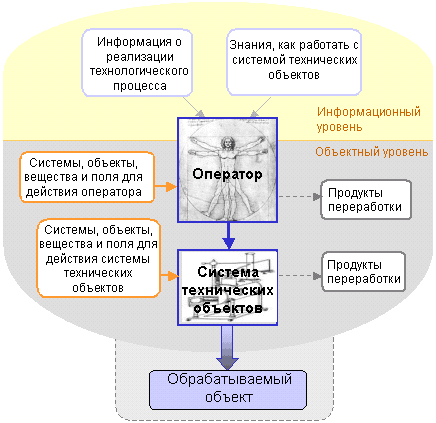
\includegraphics[width=.8\textwidth]{mts-3.png}
\end{center}
In dieser Struktur erhält die CU die Möglichkeit, überall und an jedem Ort zu arbeiten,
völlig autonom. Auch in der Schwerelosigkeit und im luftleeren Raum.

Dieser Ansatz - Ausstattung des Fahrzeugs mit allem, was für seine nutzbringende Leistung erforderlich ist
Funktion - lehnt das Traditionelle nicht ab, sondern ist sehr bequem. Sammeln Sie alles ein.
die notwendig sind, um die Funktion in einem System auszuführen und umzusetzen,
mental vom Supersystem getrennt. Es ist einfacher, jede Arbeit zu erledigen, wenn man sie vorher macht.
alle notwendigen Materialien, Werkzeuge und Zeichnungen vorzubereiten und zu arrangieren.
auf die bequemste Art und Weise, so dass Sie sich nicht um den "Workshop" kümmern müssen,
Wir müssen uns daran erinnern, was wir noch brauchen, damit unsere CU funktioniert.

Das heißt, das Technische System ist das Supersystem für das Technische System.
(materielle) Objekte.

Dieses Verständnis der TS stimmt mit ihrer Beschreibung überein, die N. Matvienko gibt.
[8]: \extbf{"Jedes technische System ist eine Reihe von realen Dingen,
 von Energie- und Informationselementen (mit anderen Worten - materielle
 Teile und Komponenten, Energieressourcen für deren Funktion und Aufbau
 Vorschriften, Anweisungen, Befehle, Signale, die die Abfolge definieren und
 Art der Interaktion realer Elemente mit umgebenden Systemen und zwischen
 von mir selbst)".

Dieser Ansatz stellt den menschlichen Bediener in den Mittelpunkt des technischen Systems.

In diesem Fall kann ein von einer Person organisiertes "Technisches System" bedeuten
die Verwendung von technischen oder natürlichen Objektelementen - zum Beispiel
Akupunktur oder Versand, und zwar ganz ohne sie - Rede
einen Anwalt vor Gericht oder einen Tanz. Das macht manchmal keinen großen Unterschied. Ein Beispiel dafür.
Ein Anwalt, der mit einem Mikrofon vor dem Saal spricht, oder
ohne ihn.

Nun, wenn man es so sieht, ist der Mann ein multifunktionaler Technischer.
Das System. Die Natur des Menschen ist zweigeteilt - er hat die Fähigkeit zu denken,
ihre Handlungen zu modellieren, Entscheidungen zu treffen. Und handeln Sie mit Ihrer
ein Gremium, das irgendeine Art von Arbeit leistet. Hier kommen sie zusammen.
Informationen und materielle Bestandteile einer Person.


Der Begriff "menschlicher Bediener" umfasst alle wesentlichen Teile des Fahrzeugs und, vorbehaltlich der Informationen
und Logistik, kann einige Funktionen erfüllen, die mit
mit den Fähigkeiten Ihres Körpers. Wenn diese Möglichkeiten ausgeschöpft sind, ist es möglich
den Körper mit materiellen Objekten zu ergänzen, sie in Systeme zu integrieren und zu erweitern
der menschlichen Fähigkeiten. Der normale Prozess des technischen Einsatzes beginnt.
Systeme. Fels, Stock, Schaufel, Bagger Der.... Mensch wird immer stärker und stärker,
mehr und mehr Arbeit leisten können.


Was ist mit der Gerinnung? Schließlich scheint sich ein Mann bereits zusammengerollt zu haben
Das ist unmöglich. Ja, wenn es um kollabierende Objekte geht. Aber es gibt eine Gerinnung.
geht auf einer informativen Ebene.

Es ist zum Beispiel an der Zeit, den Garten zu bewässern. Wir könnten die Gießkanne nehmen und den Schlauch anpassen,
um eine ganze Bewässerungsmaschine aufzustellen. Oder Sie könnten einfach in den Himmel schauen und, äh
Es wird bald regnen, Sie müssen nichts tun. Ich meine die Beschneidung.
erfolgt auf der Ebene der Funktionen, der technologischen Operationen. Schließlich, auf der Ebene
System- und Prozessgestaltung. Eine logische Fortsetzung dieser Richtung
ist die TRIZ selbst. Schließlich sind die Begriffe "perfekt", "perfekt ultimativ".
Ergebnis" ist eines der Grundkonzepte dieser Methode.

Es wurde vor langer Zeit entdeckt, und ein seltenes Märchen kommt nicht ohne etwas aus
...ist zu einer eigenen Sache geworden, ein Mann hat ohne Kosten erreicht, was er will. Mit der Kraft von .
sozusagen der Gedanke, Berge zu zerschlagen. Durch die Zeit zu reisen und
des Weltraums. "Terms of Reference" für die menschliche Entwicklung in dieser Richtung...
... Fantasten und Geschichtenerzähler verschreiben es. Und es gibt Grund zu der Annahme, dass diese
wird die Richtung gemeistert werden. Levitation, Bewegen von Objekten durch Sicht, Kommunikation über
große Entfernungen ohne technische Mittel und vieles mehr - vielleicht
für den Menschen verfügbar ist.


Ja, das ist interessant, aber was all das oben Genannte für die Transformation, die Verbesserung...
Technische Systeme in der realen Praxis?


\section*{Geringer Anstieg der Mittel, die für
Systemtransformationen.}

\mph{Die folgenden Ressourcen können für den traditionellen Ansatz verwendet werden:}.
\begin{itemize}
\item[1.] Das System selbst.
\item 2: Ihre Untersysteme.
\Position[3.] Verbindungen zwischen Subsystemen.
\Position[4.] Verbindungen zwischen den einzelnen Subsystemen und dem System.
\end{itemize}
\mph{Ausgehend von dem vorgeschlagenen Ansatz, wie viele Ressourcen genutzt werden können
 nimmt dramatisch zu. Dies sind nur einige von ihnen: }
\begin{itemize}
\item[1.] Das technische System selbst.
\2. technologisches Verfahren.
\Posten[3.] Technologische Operationen.
\Posten[4.] System technischer Einrichtungen.
\Position[5.] Subsysteme des Systems der technischen Objekte.
\Posten[6.] Operator, als denkendes System.
\item[7.] Der Körper des Operateurs ist wie ein materielles biologisches System.
\item[8.] Die Sinne des Operateurs.
\Posten[9.] System der Operator-Fähigkeiten.
\Posten[10.] Separate Operator-Fähigkeiten.
\Posten[11.] Vom System verbrauchte Systeme, Objekte, Substanzen und Felder
 technische Einrichtungen.
\Posten[12.] Systeme, Einrichtungen, Stoffe und Felder, die vom Bediener verbraucht werden.
\item[13.] Verbindungen zwischen dem technischen System und dem technologischen Prozess.
\Posten[14.] Verbindungen zwischen technologischen Operationen und technologischem Prozess
\Posten[15.] Verbindungen zwischen technologischen Operationen.
\Posten[16.] Verbindungen zwischen dem technischen System und technologischen Operationen.
\Posten[17.] Wechselwirkung zwischen Substanzen und Feldern, die vom technischen System und der
 durch ein System von technischen Einrichtungen.
\Posten[18.] Wechselwirkung zwischen Substanzen und Feldern, die vom technischen System und der
 als Betreiber.
\Position[19.] Verbindungen zwischen den Teilsystemen des Systems der technischen Anlagen.
\Position[20.] Verbindungen zwischen jedem Subsystem des materiellen Objektsystems und
 durch ein System von technischen Einrichtungen.
\Position[21.] Verbindungen zwischen den Teilsystemen des Systems der technischen Einrichtungen und
 technologischer Prozess.
\end{itemize}
........ Und viele andere Kombinationen von technischen Systemelementen.......

Es ist ein guter Zeitpunkt, um einige Beispiele zu nennen. 

\Beginn{Briefumschlag}{l}{.3extremer Breite}
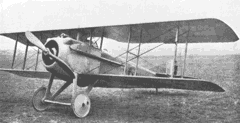
\includegraphics[width=.3\textwidth]{mts-4.png}
\nd{hüllende Figur}
\Absatz{1. Klassisches Flugzeug.}
Ein klassisches Flugzeug des frühen zwanzigsten Jahrhunderts sind die beiden Flügel, die
wurden mit zahlreichen Pfosten und Seilen am Rumpf befestigt.
eine Strecke. Damit ein Flugzeug wie dieses gut fliegen konnte (es war besonders wichtig
für Kampfflugzeuge), müssen Dehnungsstreifen richtig gespannt werden. Seit die Seile
unter Last herausgezogen wurden, mussten Dehnungsstreifen oft mit Hilfe von
des einfachsten Schraubmechanismus. An der Strecke wurde eine spezielle Schraube angebracht.
das Lineal, und die Strecke wurde mit einem Dynamometer herausgezogen. Über den Grad der Spannung.
wurden anhand der Abweichung der Strecke von der Geraden beurteilt. Dieser Prozess war sehr
mühsam und langsam.

Was ist zu tun? Wie kann der Prozess der Dehnungsstreifen-Anpassung beschleunigt werden?

Tatsächlich war es notwendig, ein neues System zu synthetisieren, um Folgendes zu regulieren
eine Strecke. Wenn die einzigen Leute, die das tun würden, aus dem System kämen.
Das Material Objekte, die benutzt werden, um diese Funktion zu erfüllen und sie dann zu lösen
wäre extrem schwierig. Wenn Sie sich erinnern und bedenken, dass es ein System gibt...
Operator, dann ist die Anzahl der möglichen Transformationen signifikant
nimmt zu. Sie können das Problem also mit den Sinnen des Bedieners lösen.

\Beginn{Briefumschlag}{l}{.1externe Breite}
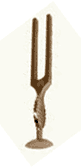
\includegraphics[width=.1\textwidth]{mts-5.png}
\nd{hüllende Figur}
Wirklich, warum nicht das Gehör nutzen, oder besser gesagt, Menschen mit einem hohen
mit tonalem Gehör? Klavierstimmer wurden eingeladen, die Dehnung anzupassen,
der Anpassungsprozess wurde um ein Vielfaches beschleunigt.

Da Klavierstimmer nicht genug waren, mussten wir interessanterweise
die folgende Lösung, die die in der TRIZ wiederholt beschriebene nachzeichnet
Trend: "Verdrängung der CU". Die Dehnungskontrolle wurde wieder angeordnet...
zur Mechanik, sondern anstelle eines schwerfälligen Lineals und Dynamometers.
eine ordnungsgemäß eingerichtete Kamera zu verwenden.

\Absatz{2. Die Öllampe.}
Es ist schwer vorstellbar, welche titanische Arbeit die Erfinder geleistet haben,
und versuchen, die Öllampe zum Leuchten zu bringen. Das ganze Problem war mit den schlechten
Ölversorgung der Dochtspitze. Um den Fluss zu verbessern, haben zahlreiche
Federvorrichtungen, die Druck im Ölbehälter erzeugen. Verwendet .
sowie Pumpen für die erzwungene Ölversorgung. Ich meine, die Arbeit war im Rahmen
"technische Anlagensysteme" - versuchte, die Maschine zu verbessern. 
Und als wir die vollständige Zusammensetzung der CU betrachteten, wurde klar, dass es bei der Frage nicht um
und in brennbarem Material. Wenn statt schlecht absorbiert.
Der Öldocht verwendete fließendes Kerosin, alle Probleme waren verschwunden. 

\Absatz{3. Computer.}
Angenommen, Sie möchten Ihren Computer im Dunkeln benutzen. Wenn wir
das System der materiellen Objekte zu transformieren, dann kommt sofort die Idee
Leuchttasten, Glühbirnen und so weiter. Wenn Sie über das technische System nachdenken,
dann liegt die Antwort auf der Hand - der Bediener muss in der Lage sein, im Dunkeln zu drucken, denken Sie daran.
Tastenanordnung auswendig.


Was kann ich zum Schluss sagen? Jetzt in TRIZ und anderen innovativen Methoden.
die Begriffe "technisches System", d.h. das System, sind völlig verworren,
\extbf irgendeine Funktion ausübt, und "Technisches (materielles) System".
Objekte", d.h. das System, das extbf entworfen wurde, um eine Art von
Funktionen. Indem man sich so wenig wie möglich in das Argument der "spitzen Punkte" einmischt und
"dumb-tips" (siehe Inschrift), habe ich versucht, es herauszufinden.

Ohne den Leser auffordern zu wollen, mir zuzustimmen, würde ich mich freuen, wenn dieser Analyseversuch
wird sich für ihn als nützlich erweisen.

Ich bin den Kollegen V. Lenyashin, G. Severinets, E. Novitskaya, N. Khomenko sehr dankbar.
und kritisiert schonungslos die erste Version des Artikels an W. Sibirjakow für seine Hilfe bei
Vorbereitung dieses Materials.
\section*{Literatur}
\begin{itemize}
\item[1.] B.R. Gaines. "Allgemeine Systemforschung: Quo vadis?" Allgemeines System.
 Jahresschüler, 24, 1979.
\item 2: A.A. Bogdanov. Allgemeine Organisationswissenschaft. Tektologie. Buch 1 -
 М., 1989. - – С. 48.
\item 3: G.S. Altschuller. Kreativität als exakte Wissenschaft.
 \url{http://www.trizminsk.org/r/4117.htm#05}.
\item 4: A.F. Kamenev. Technische Systeme. Regelmäßigkeiten der Entwicklung.
 Leningrad, "Mashinostroenie", 1985.
\item 5: G. Altschuller, B. Zlotin, A. Zusman. V. Filatov. Suche nach neuen Ideen: von
 Einblicke in die Technologie. Chisinau, Carta Moldaveniasca, 1989. p. 365.
\item 6. V. Korolev. Über den Begriff "System". Enzyklopädie der TRIZ.
 \url{http://triz.port5.com/data/w24.html}.
\item 7: V. Korolev. Über den Begriff "System" (2). Enzyklopädie der TRIZ.
 \url{http://triz.port5.com/data/w108.html}.
\Posten[8.] N.N. Matvienko. Begriffe der TRIZ (Problemsammlung). Wladiwostok,
 1991.
\item 9: Y.P. Salamatov. Gesetzessystem der Technikentwicklung (Grundlagen der Theorie der Zukunft).
 Entwicklung technischer Systeme). INSTITUT FÜR INNOVATIVE GESTALTUNG. Krasnojarsk,
 1996. \url{http://www.trizminsk.org/e/21101000.htm}.
\item 10: V.A. Sviridov. Menschlicher Faktor.
 \url{http://www.rusavia.spb.ru/digest/sv/sv.html}.
\item 11: G.I. Iwanow. Formeln der Kreativität oder wie man lernt
 zu erfinden. Moskau. "Aufklärung". 1994
\item 12: F. Cooper. Prärie. 
\end{itemize}

\end{document}
